\documentclass[a4paper,11pt,oneside]{book}

\usepackage[utf8]{inputenc}
\usepackage[T1]{fontenc}
\usepackage[italian]{babel}
\usepackage{amsfonts,amsmath,amssymb,amsmath,amsthm,color}
\usepackage{graphicx}
\usepackage{float}
\usepackage{emptypage}
\usepackage{titlesec}
\usepackage{algorithm,algcompatible}
\usepackage{tabularx}
\usepackage[nottoc]{tocbibind}
\usepackage{subcaption}
\usepackage[backend=bibtex,style=ieee,sorting=none]{biblatex}
\usepackage[hidelinks]{hyperref}
\usepackage{filecontents}
\usepackage{csquotes}
\usepackage[font=small,labelfont=bf]{caption} % caption belle alle figure

%Stile per l'indice
\renewcommand{\chaptermark}[1]{\markboth{#1}{}}
\renewcommand{\tocetcmark}[1]{\markboth{#1}{}}
\renewcommand{\sectionmark}[1]{\markright{\thesection\ #1}}

% Stile dei titoli dei capitoli
\definecolor{gray75}{gray}{0.75}
\newcommand{\hsp}{\hspace{20pt}}
\titleformat{\chapter}[hang]
{\Huge\bfseries}
{\thechapter\hsp\textcolor{gray75}{|}\hsp}
{0pt}
{\Huge\bfseries}

% Bibliografia
\bibliography{./bibliografia/bibliografia} % put your bibliography here

\setcounter{tocdepth}{1}
\raggedbottom

\graphicspath{{./immagini/}}

\begin{document}
	


%%%%%% First Page %%%

\pagestyle{myheadings}


\thispagestyle{empty}  
                                               
\begin{center}                                                            
    \vspace{2mm}
    {\large ALMA MATER STUDIORUM -- UNIVERSIT\`A DI BOLOGNA} \\  
                         
      \vspace{2mm}
\end{center}

\begin{center}
      \vspace{5mm}
      {\large \uppercase{Scuola di Ingegneria e Architettura}} \\
        \vspace{5mm}
       {\large Dipartimento di Informatica\\
       Scienza e Ingegneria }\\
   		{\large DISI}\\
        \vspace{5mm}
      {\Large \bf Corso di Laurea in Ingegneria Informatica}\\
      \vspace{5mm}
      %{ \textbf{Master Thesis}\\ in\\ \textit{Distributed Control Systems}}\\
      \vspace{5mm}
      {\LARGE\bf Title} \\                
      \vspace{15mm}
      
      % table??
		\begin{tabularx}{\textwidth} 
      { 
				>{\raggedright\arraybackslash}X 
				>{\raggedleft\arraybackslash}X }
				{\large Candidato: } & {\large Relatore:} \\[3mm]
				{\large \itshape Gianmiriano Porrazzo  } & {\large \itshape prof. Andrea Camisa} \\[3mm]
				& {\large Correlatore: } \\[3mm] 
				& {\large \itshape prof. Andrea Testa}
    \end{tabularx}
      \vfill
      {\large Anno Accademico \\ \itshape 2021--2022} \\
      \vspace{5mm}
      {\large Sessione \\ \itshape II}
\end{center}


\vfill

\newpage
\thispagestyle{empty}



%%%%%%FRONTESPIZIO%%%%%%



%%%%%% INDICE %%%%%%%%%%

\tableofcontents


%%%%%% ABSTRACT %%%%%%%%%%


\chapter*{Abstract}
\addcontentsline{toc}{chapter}{Abstract}

L'uso di tecniche di machine learnig è molto
%%%%%%% BODY %%%%%%%%%

\chapter*{Introduzione}
\addcontentsline{toc}{chapter}{Introduzione}
Il machine learning ha vari campi applicativi.
Uno di questi è quello di riconoscere dei pattern in modo che tali algoritmi possano apprendere e fare predizioni su un insieme di dati.

Un settore sul quale gli algoritmi di machine learning sono molto applicati è quello della medicina.
In questo documnento si tratterà di come usare gli algoritmi di machine learning per fare predizioni su un dataset che contiene dati relativi a pazienti affetti da Covid-19.

Esistono vari modi per analizzare i dati e fare apprendere la rete neurale in modo che le predizioni da essa effettuate abbiano senso.
Tali metodologie possono variare per via dei dati che compongono il dataset, ma anche dal tipo di previsioni che la rete deve effettuare.

L'algoritmo usato consiste in una rete neurale artificiale.
Tale rete è composta da vari neuroni, i quali hanno il compito di prendere dei dati in input, apprenderne le caratteristiche principali e sulla base di ciò effettuare le previsioni.

I neuroni che si occupano dell'apprendimento sono organizzati in vari layer nascosti. Ogni layer è composto da uno o più neuroni che interagiscono tra di loro. 

Come già accennato in base al tipo di dato da studiare si può prediligere una tipologia di rete ad un'altra.
Nel caso di questa tesi si è scelto di usare una rete neurale convoluzionale (CNN-\emph{Convolutional Neural Network}) per apprendere dalle immagini e una MLP ( \emph{Multi-Layer Perceptron} ) per gestire i metedati relativi alle immagini.




%\markboth{}{INTRODUZIONE}
	
%	\section*{Motivazioni}
%	\addcontentsline{toc}{section}{Motivazioni}
	
%  (articoli e references)
		
%	\section*{Letteratura}
%	\addcontentsline{toc}{section}{Letteratura}
	
	
%	\section*{Contributi}
%	\addcontentsline{toc}{section}{Contributi}
	
%	\section*{Organizzazione}

%%%%%%% CAPITOLI %%%%%%%%%

\chapter{Strumenti usati}
\label{ch:Strumenti usati}

Esistono vari framework per lo sviluppo di reti neurali, uno dei più usati è TensorFlow \cite{tsf}. 
\\
TensorFlow presenta modelli già creati e allenati, i cui pesi possono essere presi per sfruttare tale modello.
Insieme all'uso di altre librerie come Keras l'implementazione di una rete neurale che gestisca i dati a disposizione 
è molto semplificato.
\\
La rete di base usata per partire con l'analisi delle immagini è la MobileNetV2. Tale rete è una CNN che, prendendo come input delle 
immagini.
A tale rete, tuttavia, sono state apportate delle modifiche per via delle dimensioni dell'input e della tipologia di dato 
che si vuole ottenere come previsione.
\\
Oltre a questa tipologia di rete si è sfruttata anche una U-Net, al fine di omogeneizzare tutte le immagini che vengono date come input della MobileNetV2.
La U-Net usata è EfficientNet, con dei pesi preallenati per riconoscere immagini simili a quelle presenti nel dataset di riferimento.


\chapter{Dataset}
\label{ch:Dataset}
\section{Composizione}
*inserire link all'hackaton e immagini dataset*
\\\\
Il dataset usato per effettuare lo studio è stato preso da un hackaton riguardante la creazione di una rete neurale in grado di apprendere 
da immagini relative a radiografie di pazienti affetti da covid in modo da predirre la gravità della prognosi.
\\\\
Dunque il dataset usato è formato da immagini raffiguranti radiografie dei polmoni, le quali tuttavia non sono omogenee. Per tale motivo 
si è dovuto effettuare un passaggio preliminare in modo da rendere le immagini tutte della stessa dimensione, ma non distorcendole.
\\\\
Oltre alle immagini sono presenti anche un insieme di metadati riguardanti lo stato in cui il paziente è entrato all'ospedale e l'anamnesi dello stesso.
Tali metadati presentano descrivono varie informazioni relative al paziente, per tale motivo sono rappresentate anche in modo diverso: esistono dati di tipo categorico, sia con più categorie che con
due sole categoria, dati che possono essere considerati come booleani e dati interi, come ad esempio l'età.
\\\\
\section{Immagini}
Dando uno sguardo alla composizione del dataset si può notare come le immagini risultano avere dimensione diversa. Per tale motivo 
risulta utile eseguire un preprocessing delle immagini, in cui si effetuano vari passaggi:
\begin{itemize}
    \item Riconoscere i polmoni e crearne una mascehera
    \item Ricavare una bounding-box che contenga i polmoni
    \item Ritagliare la bounding-box contenente i polmoni, in modo che abbiano tutte la stessa dimensione
\end{itemize}

È importante sottolineare che nell'eseguire tali passaggi si necessita di evitare di distorcere l'immagine, per tale 
motivo si faranno considerazioni sull'aspect ratio dell'immagine. 
\\\\
Tali passaggi serviranno per ottenere immagini omogenee, in grado di consentire alla rete di identificare i polmoni ed avranno 
una dimensione pari a 224 x 224
\section{U-Net}
Al fine di effettuare il riconoscimento dei polmoni allinterno dell'immagine, si sfrutta una U-Net.
Una U-Net è una rete convoluzionale sviluppata per eseguire la segmentazione dell'immagine. Il processo di segmentazione consiste nell'assegnare ad 
ogni gruppo di pixel selezionato una categoria. Ad esempio si potrebbe avere un insieme di pixel del'immagine che identificano il contorno dei polmoni.
\\\\
Lo scopo della U-Net è dunque quello di prendere in input l'immagine e creare una maschera che raffiguri i polmoni.
La maschera è un'immagine formata da pixel con valore in [0,1] e mira a creare un'immagine raffigurante la distinzione tra cosa rappresenta 
i polmoni e cosa rappresenta lo sfondo.
L'utilià della maschera è quella di consentirci di trovare con maggior facilità la bounding box.
\\\\
La rete usata per la segmentazione è EfficientNet. Tale rete prende un input di dimensione predefinita e restituisce un'immagine della stessa
dimensione, rappresentante la maschera. Nel caso considerato, inoltre si è deciso di usare come funzione di attivazione Sigmoid e di sfruttare 
i pesi preallenati su ImageNet, per avere maggior precisione.
\\\\
Essendo le immagini di dimensione diversa, prima di darle in input alla rete viene effettuato un ridimensionamento alle dimensioni accettate dalla rete. 
Tale passaggio viene effettuato mantenendo l'aspect ratio dell'immagine e inserendo padding nero per evitare distorsione.
L'aspect ratio rappresenta il rapporto tra le dimensioni dell'immagine, per evitare distorsione della stessa, si deve conseravre tale rapporto.
Nel caso in cui l'immagine non soddisfi i requisiti delle nuove dimensioni si procede con l'aggiunta di padding di colore nero, ovvero si inseriscono i pixel necessari 
all'immagine per raggiungere la dimensione necessaria usando un colore non influente. 
\\\\
La rete performa molto bene con immagini di dimensioni piccole, tuttavia si è potuto notare, a seguito di esperimenti, che nel caso considerato, la rete 
performa meglio con immagini, in input, di dimensione 256 x 256 rispetto a quelle di dimensione 224 x 224.
Per tale motivo, a seguito della segmentazione dovrà essere effettuato un ridimensionamento dell'immagine.

\section{Bounding-box}
Ottenute così le maschere retive alle immagini, queste sono alla base della costruzione delle bounding-box.
La bounding-box rappresenta il riquadro di dimensione minima, contenente i polmoni.
Per trovare tale riquadro si usano i punti estremi delle maschere: si cercano il punto più alto, più basso, il più a destra e l'estremo a sinistra.
Tali punti rappresentano le coordinate di una box, la quale conterrà per certo i polmoni.
\\\\
Avendo ora le bounding box, l'ultima cosa da fare è ritagliare le dalle immagini originali le bounding-box e ridimensionarle a 224 x 224.
È necessario in questi passaggi di ridimensionamento mantenere presente che l'aspect-ratio deve essere conservato, per cui si effettua nuovamente padding ove necessario.
\\\\
Alla fine di tale procedimento si sono ottenute delle immagini raffiguranti i polmoni e della dimensione desiderata.

\section{Metadati}
Per quanto riguarda i metadati la situazione è meno complessa, poichè gestita mediante file csv.
Innanzitutto ciò che si vuole ottenere è un insieme di dati che sia completamente pieno, ovvero presenti corrispondenze 
per tutte le righe e colonne del dataset.
Dunque si cerca di ridurre il dataset di partenza nel più grande sottinsieme che contenga tutte le corrispondenze.
Tale omogeneità deve essere presente sia nel dataset di training che in quello di test. Oltre a ciò, alla fine, si cerceranno le collonne comuni 
ai due dataset, scartando le altre. In tal modo si possono unire i due dataset così da formarne uno solo.
\\\\ 
Per iniziare si eliminano le colonne che non presentano alcun dato, o che presentano dati solo per un numero molto ristretto di paziente, per :
\begin{itemize}
    \item nel dataset di training sono state scartate le colonne
    \begin{itemize}
        \item giorni di febbre, 
        \item fibrina, 
        \item glucosio, 
        \item PCT, 
        \item LDH, 
        \item INR, 
        \item D\_dimer, 
        \item percentuale di ossigeno, 
        \item PaO2, 
        \item SaO2, 
        \item PaCO2, 
        \item pH, 
        \item cardiopatia ischemica,
        \item insufficienza respiratori,
        \item obesità, 
        \item positività all'ammssione, 
        \item temperatura corporea, 
        \item RBC, 
        \item CRP.
    \end{itemize} 
    \item nel dataset di test sono state scartate le colonne
    \begin{itemize}
        \item giorni febbre, 
        \item fibrina, 
        \item LDH,
        \item PaO2,
        \item PaCo2, 
        \item pH, 
        \item PCT, 
        \item INR,
        \item D\_dimer, 
        \item SaO2, 
        \item tempertaure corporea, 
        \item CRP.
    \end{itemize} 
\end{itemize} 

Eliminate le colonne in eccesso, si procede con l'eliminazione dei paziente che non presentano tutti i dati.
A seguito di tale operazione le righe, ovvero i pazienti, che sono presenti nel dataset di train sono 946, mentre quelle del dataset di test
472.
Le colonne in comune tra i due dataset sono:
\begin{itemize}
    \item Ospedale, 
    \item Età, 
    \item Sesso,
    \item Tosse, 
    \item Difficoltà respiratorie
    \item Numero di cellule bianche,
    \item Pressione sanguigna alta,  
    \item Diabete,
    \item Demenza,  
    \item BPCO (Broncopneumopatia cronica ostruttiva),
    \item Cancro, 
    \item Malattia renale cronica
\end{itemize}

In tal modo si è ottenuto un dataset che contiene 12 colonne significativa (sopra elencate) contenenti dati per 
1418 pazienti.


\chapter{Risultati training con sole immagini}
\label{ch:CNN}
\section{Creazione rete neurale}
Lo sviluppo della rete neurale convoluzionale, per effettuare previsioni partendo dalle immagini, è basata sulla rete 
MobileNetV2. L'uso di tale rete come base consente di usare dei pesi preallenati in modo da rendere il processo di training sul dataset più efficiente.
\\\\
Tuttavia tale processo necessita di alcune fasi aggiuntive per fare in modo che la rete riesca a prendere i dati della dimensione esatta 
e restituire delle previsioni nell'insieme desiderato.
\\\\
Tali operazioni sono:
\begin{itemize}
    \item Inserire la dimensione delle immagini nel layer di input
    \item Effettuare fine tuning e transfer learning per poter usare i pesi preallenati 
    \item Inserire dei layer finali per ottenere degli output significativi
\end{itemize}

La dimensione scelta delle immagini è (224x224), dunque la rete prende in ingresso degli array di dimensione 224x224x3 (dove quest'ultimo indica l'uso dei colori RGB).
Per tale motivo il layer di input deve accettare tale dimensione.
\\\\
I pesi preallenati che si sono scelti sono pesi allenati su ImageNet. ImageNet è un dataset di immagini suddivise in 1000 classi. Il dataset su cui si deve svolgere il training, tuttavia, possiede 
unicamente una classe, per via del fatto che abbiamo trasformato il valore della prognosi da una string ad un valore binario. 
Per cui l'immagine può appartenere o meno a tale classe.
\\\\
Al fine di poter usare tali pesi per effettuare il training, si necessita dunque di ulteriori passaggi: 
\begin{itemize}
    \item Transfer Learning
    \item Fine tuning
\end{itemize}

\section{Transfer Learning}

Il transfer learning consente di sfruttare la rete già allenata a risolvere problemi diversi, ma comunque correlati con quello di interesse.
Nel caso considerato tale tecnica permette di usare una rete allenata per prevedere l'appartenenza di una immagine ad una delle 1000 classi di ImageNet
per creare una rete in grado di classificare le immagini del dataset in una unica classe.
\\\\
Per sfruttare la rete allenata, congeliamo lo stato dei layer di classificazione, al fine di non alterarli, e settiamo la rete come non allenabile.
In tal modo si è ottenuto un nuovo modello basato sulla MobileNetV2.
\\\\
Ora si presenta un problema relativo alla classificazione. Per ovviare al fatto che tale operazione sarà fatta per una sola classe, si necessita dell'inserimento di altri layer alla fine del modello precedentemente ottenuto.
\\\\
Tali layers sono:
\begin{itemize}
    \item un GlobalAveragePooling2D()
    \item due Dense() 
\end{itemize}  
$\\\\$
Il primo layer serve per via del fatto che allo stato attuale la rete produce un output multidimensionale e, per ottenere previsioni formate da un singolo vettore 
della dimensione prevista, usiamo tale layer, il quale genera previsioni basate sul blocco multidimensionale e facendone una media.
\\\\
Il primo Dense layer viene usato per generare l'output prodotto dalle immagini dei polmoni. Tale layer è formato da 100 neuroni ed ha come funzione di attivazione ReLu.
\\\\
Il secondo Dense layer svolge il lavoro di classificazione vero e proprio. Per via del fatto che si è scelto di usare una label binaria, ovvero classifichiamo su un'unica classe, tale 
layer è composto da un solo neurone, ed ha come funzione di attivazione Sigmoid.
\\\\
Una volta creati i layers, per completare la fase di transfer learning, si deve compilare il modello finale, ottenuto aggiungendo i nuovi layers.
\\\\
Ora la rete è pronta per una prima fase di training. In tale fase sono stati usati i seguenti parametri per il training:
\begin{itemize}
    \item Loss function: Adam
    \item Metrica: accuracy
    \item Epoche 150
    \item Batch size: 30
\end{itemize}
\clearpage
\section{Risultati dei test effettuati per il transfer learning}
Per quanto concerne il valore del learning rate sono si è deciso di effettuare prove sia con $10^{-3}$ che con 
$10^{-4}$.
I risultati ottenuti dal training sono espressi nei seguenti grafici.

\begin{figure}[h]
    \centering
    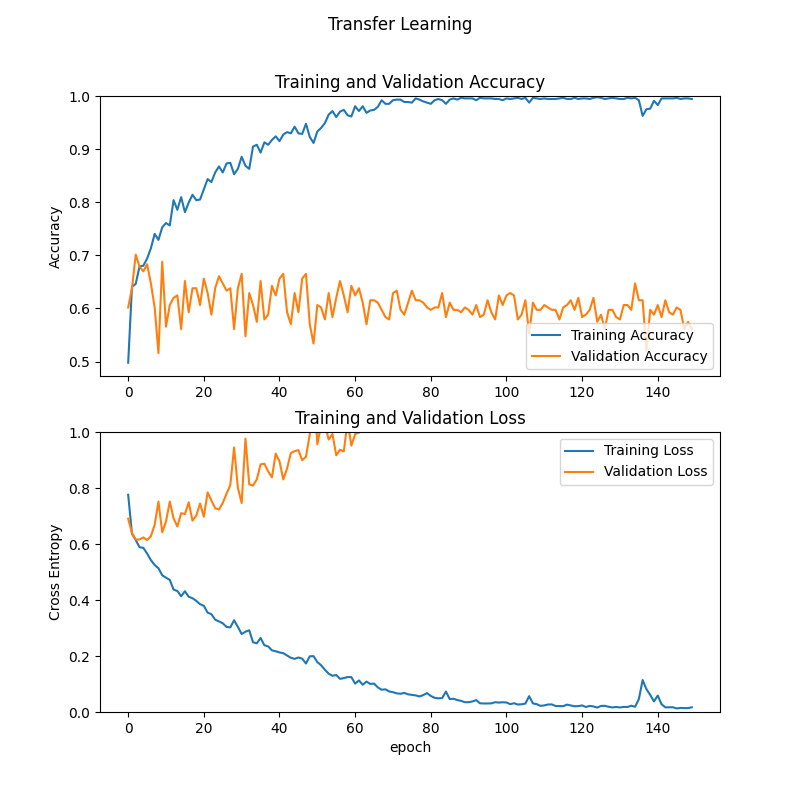
\includegraphics[width=10cm]{./10-3_150.png}
    \label{ 10^{-3} tl}
    \caption{Test effettuato usando come learning rate $10^{-3}$}
\end{figure}
\begin{figure}[h]
    \centering
    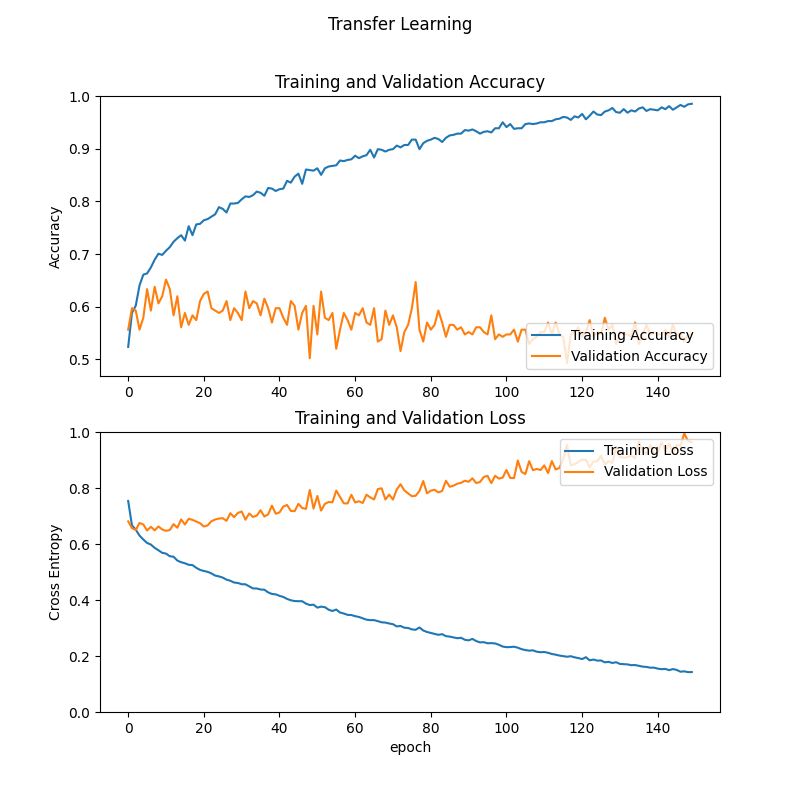
\includegraphics[width=10cm]{./10-4_150.png}
    \label{10^{-4} tl}
    \caption{Test effettuato usando come learning rate $10^{-4}$}
\end{figure}
\vspace{5000mm}
$\\\\$
Dai grafici si può notare come il training effettuato con learning rate pari a $10^{-3}$ risulta essere più preciso, 
anche se non di molto. Possiamo inoltre notare come la training loss diminuisce suggerendo il corretto funzionamento della
rete.

\section{Fine Tuning}

Per procedere con la fase di fine tuning, si deve rendere nuovamente allenabile il modello creato, 
in modo tale che i pesi possano essere allenati considerando i nuovi layers.
Così facendo si permette ai pesi di regolarsi sul dataset d'interesse, partendo da quello su cui sono stati inizialmente allenati.
\\\\
Essendo gli ultimi layers di una rete inutili in termini di classificazione, possiamo decidere di 
congelarli, ovvero non considerarli durante il training, in modo da risparmiare risorse.
Effettuato tale passaggio si può procedere con la compilazione del modello ottenuto e procedere con il training.
\\\\
I parametri relativi al training in questa fase sono:
\begin{itemize}
    \item Loss function: Adam
    \item Metrica: accuracy
    \item Epoche 30
    \item Batch size: 30
\end{itemize}
\section{Risultati dei test effettuati per il fine tuning}
$\\$
Di seguito sono riportati i risultati ottenuti a seguito del transfer learning e fine tuning, sempre considerando 
i due valori scelti per il learning rate.

\begin{figure}[htp]
    \centering
    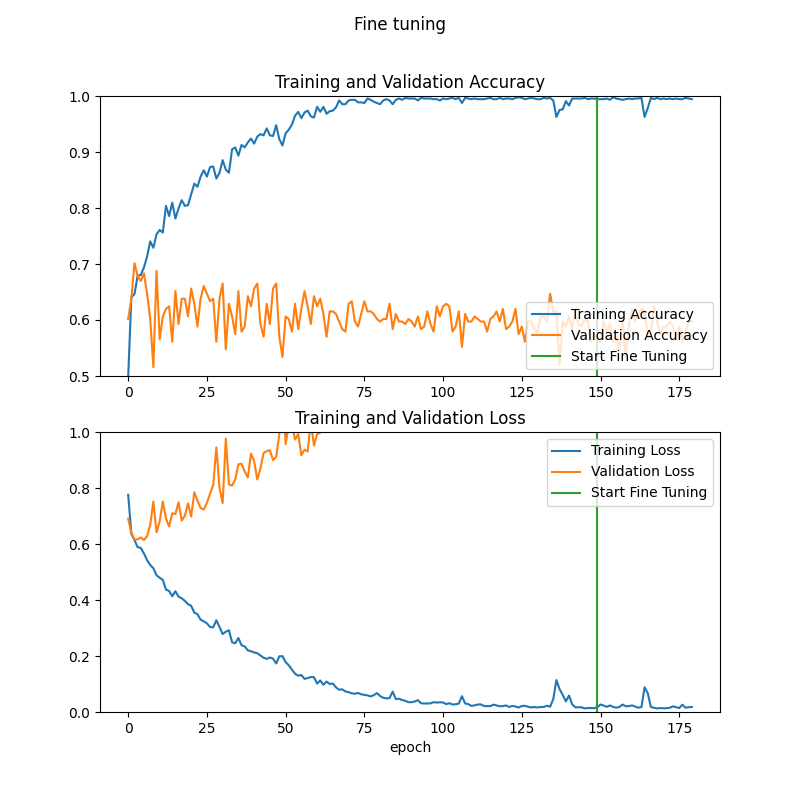
\includegraphics[width=10cm]{./10-3_150_2.png}
    \label{ 10^{-3} ft}
    \caption{Test effettuato usando come learning rate $10^{-3}$}
\end{figure}

\begin{figure}[t]
    \centering
    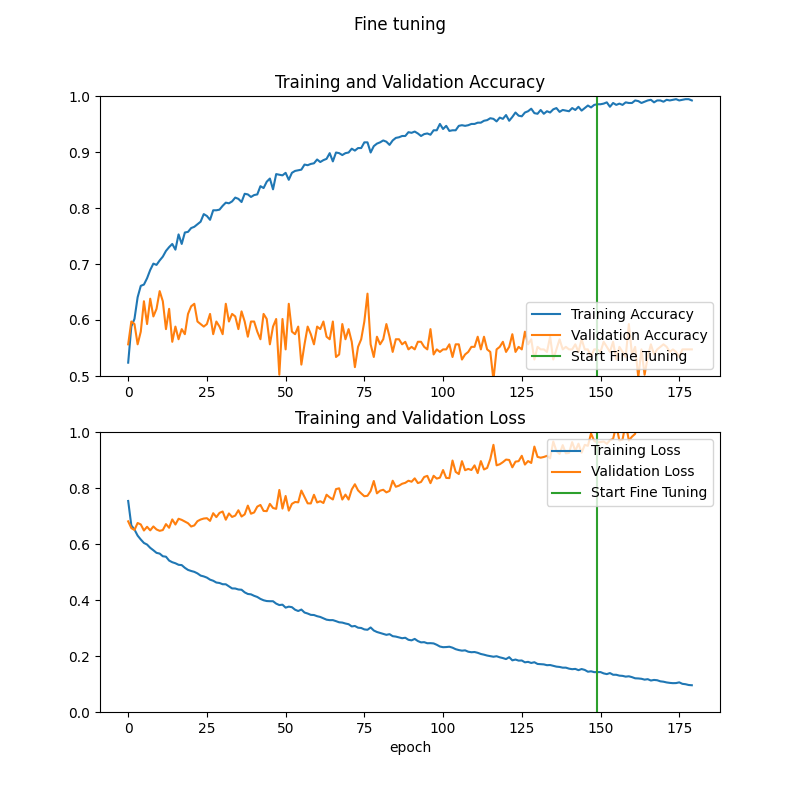
\includegraphics[width=10cm]{./10-4_150_2.png}
    \label{10^{-4} ft}
    \caption{Test effettuato usando come learning rate $10^{-4}$}
\end{figure}
\vspace{1000mm}
$\\\\$
Anche dal grafico relativo al fine tuning si una validation accuracy maggiore usando un learning rate pari a
$10^{-3}$. Importante è notare la linea verde che demarca l'inizio del fine tuning e la fine del transfer learning.

\section{Overfitting e Data Augmentation}
Dai risultati ottenuti risulta evidente la presenza di overfitting nella rete.
Tale problema si è potuto notare per via del fatto che, anche a seguito del fine tuning, la validation accuracy tende 
a diminuire.
\\\\
L'overfit può essere causato dal fatto che la rete si abitui agli input del training set, o al 
fatto che questi siano molto simili tra di loro e risponda in maniera casuale a nuovi dati. Per tale motivo si è scelto di usare la data augmentation come tecnica risolutiva.
La data augmentation consiste nel prendere le immagini del dataset, effettuare delle modifiche ad esse (come rotazioni), per 
creare una immagine nuova, in modo da introdurre diversità all'interno del dataset. 
\clearpage
$\\\\$
Per implementare tale tecnica si è optato per l'uso del ImageDataGenerator(). L'adozione di tale funzionalità presente in 
TensorFlow è dovuta al fatto che consente di creare immagini partendo dal dataset iniziale, applicando trasformazioni casualmente, scegliendo tra 
quelle selezionate.
\\\\
Le trasformazioni che sono state scelte, in base alla possibilità che la rete consideri anche le nuove immagini come 
valide, sono la rotazione verticale ed orizontale, specificando anche il range di angolo in cui effettuare tale rotazione.
La scelta di queste trasformazioni è stata validata anche osservando le immagini prodotte e riflettendo sul fatto che fossero 
sensate come input della rete.
\begin{figure}[h]
    \centering
    \begin{subfigure}{.45\textwidth}
        \centering
        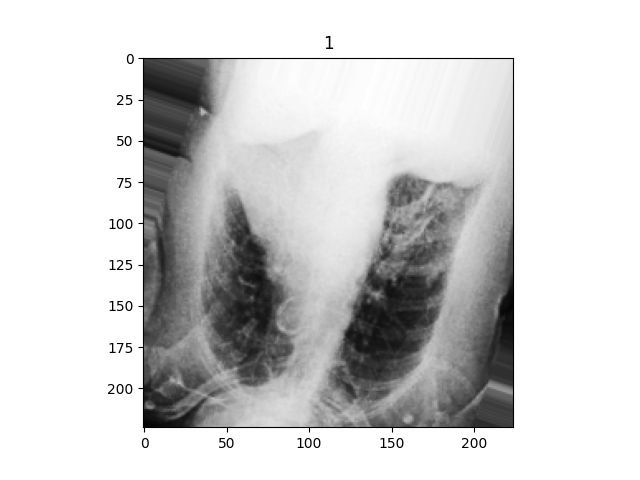
\includegraphics[width=1.25\linewidth]{augmented_ex.png}  
        %\caption{}
        \caption{SEVERE}
    \end{subfigure}
    \begin{subfigure}{.45\textwidth}
        \centering
        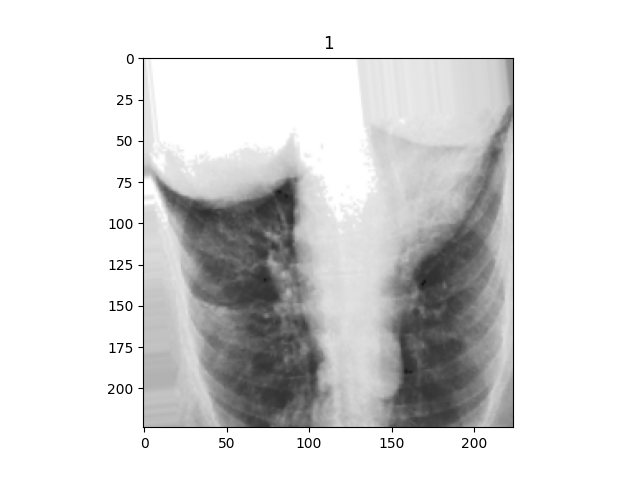
\includegraphics[width=1.25\linewidth]{augmented_ex_1.png}  
        %\caption{}
        \caption{SEVERE}
    \end{subfigure}
    \begin{subfigure}{.45\textwidth}
        \centering
        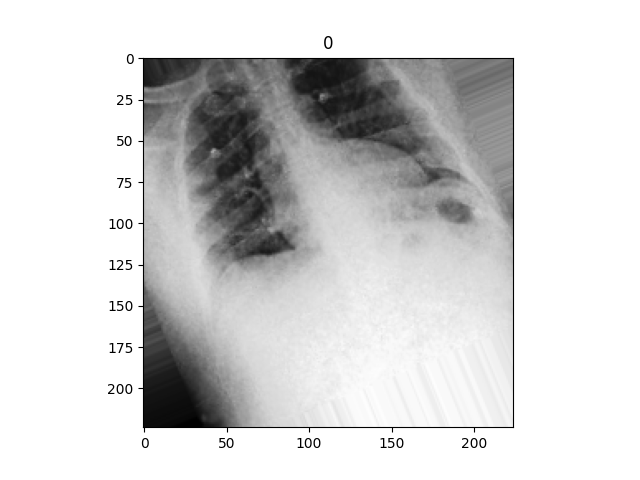
\includegraphics[width=1.25\linewidth]{augmented_ex_2.png}  
        %\caption{}
        \caption{MILD}
    \end{subfigure}
    \begin{subfigure}{.45\textwidth}
        \centering
        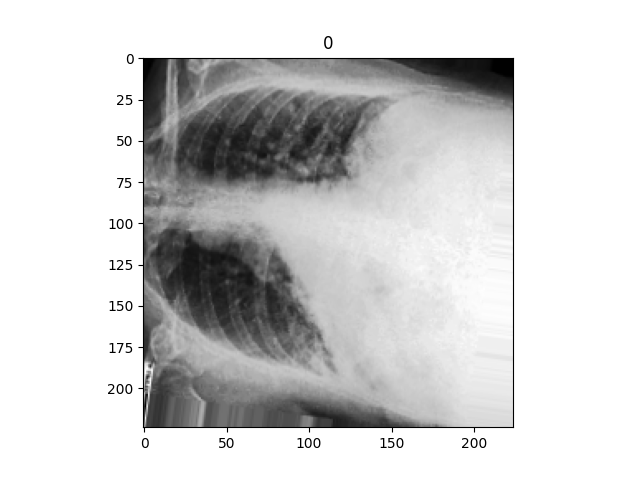
\includegraphics[width=1.25\linewidth]{augmented_ex_3.png}  
        %\caption{}
        \caption{MILD}
    \end{subfigure}
    \caption{Immagini a seguito dell'augmentation, con relativa label}
    \label{Augmentation}
\end{figure}
\\\\
È importante sottolineare che l'augmentation viene effettuata unicamente sul training set.
$\\\\$
\section{Risultati dei test effettuati per la data augmentation}
Per verificare se la data augmentation ha avuto effetto si procede con dei training della rete.
Tali training sono stati effettuati mantenendo gli stessi parametri precedentemente usati.

\begin{figure}[h]
    \centering
    \begin{subfigure}{.60\textwidth}
        \centering
        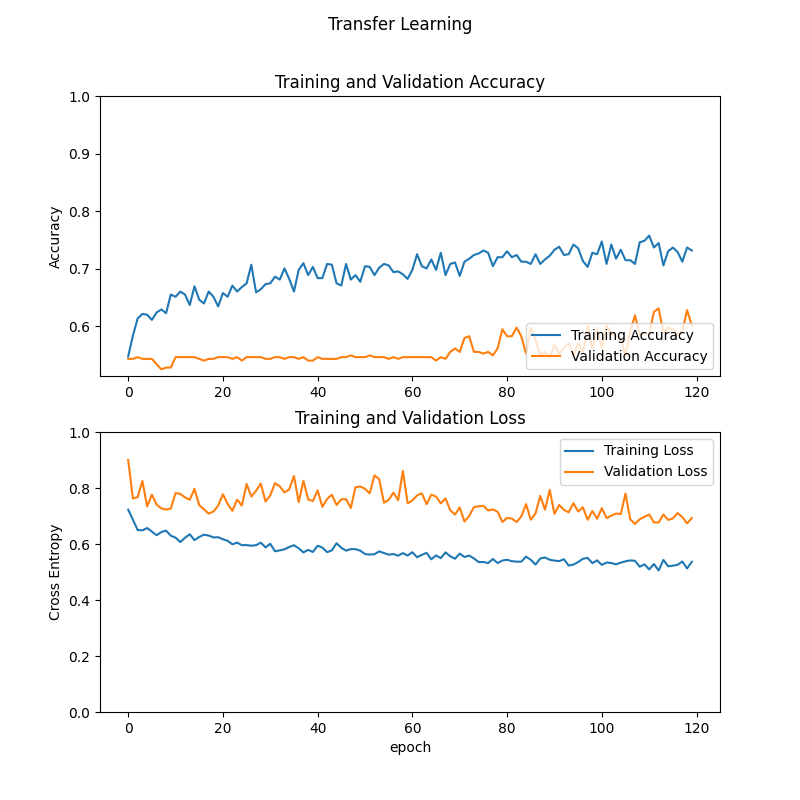
\includegraphics[width=.95\linewidth]{lr10-31_r.png}  
        %\caption{}
        %\label{SUBFIGURE LABEL 1}
    \end{subfigure}
    \begin{subfigure}{.60\textwidth}
        \centering
        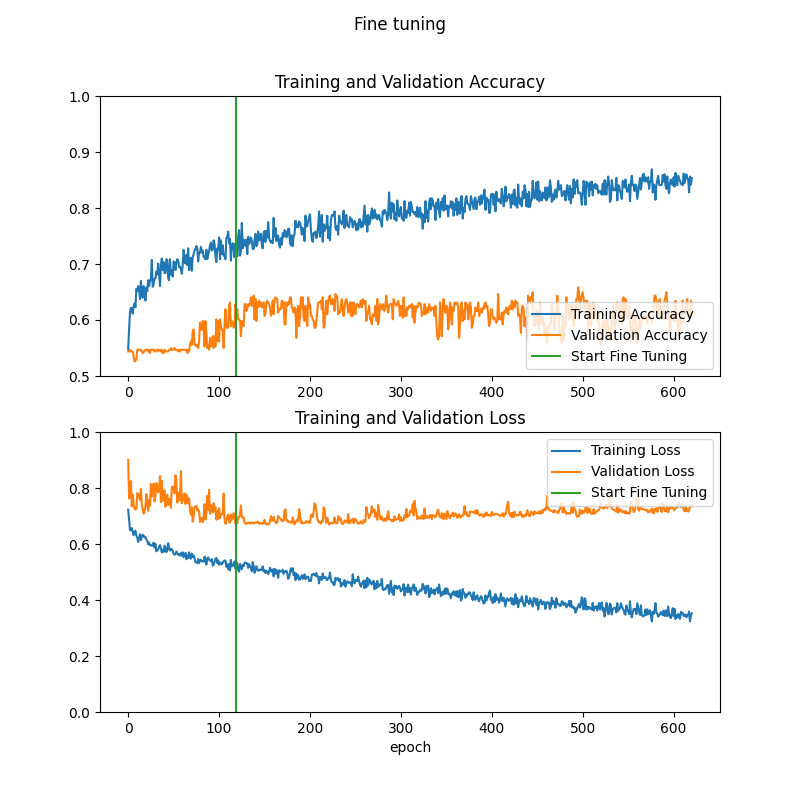
\includegraphics[width=.95\linewidth]{lr10-32_r.png}  
        %\caption{}
        %\label{SUBFIGURE LABEL 2}
    \end{subfigure}
    \caption{Training effettuato con learning rate pari a $10^{-3}$ a seguito dell'augmentation}
    \label{Training Augmentation 1}
\end{figure}
\begin{figure}[htp]
    \centering
    \begin{subfigure}{.60\textwidth}
        \centering
        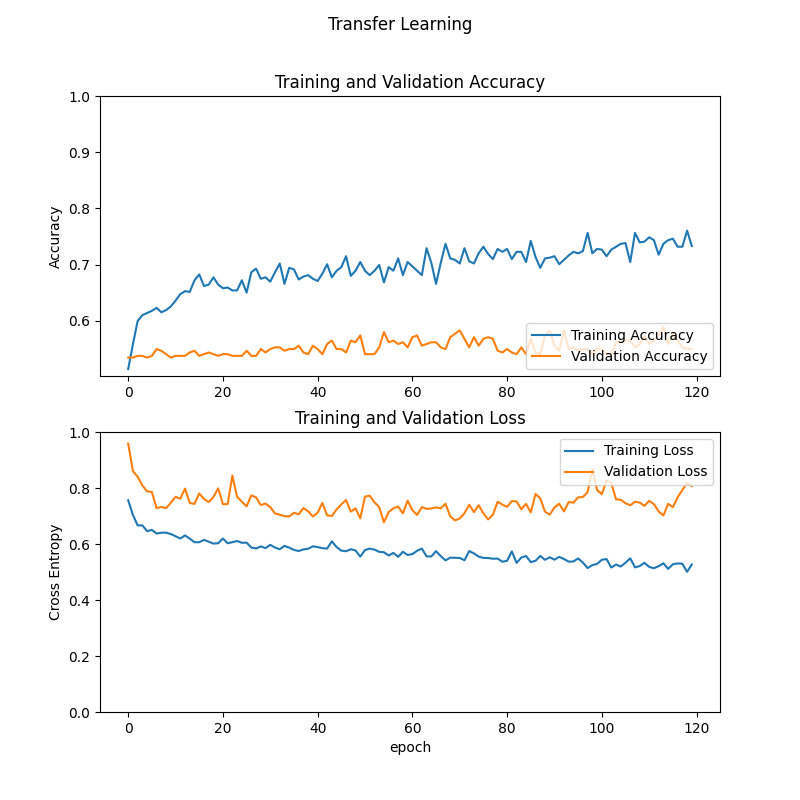
\includegraphics[width=.95\linewidth]{lr10-41_r.png}  
        %\caption{}
        %\label{SUBFIGURE LABEL 3}
    \end{subfigure}
    \begin{subfigure}{.60\textwidth}
        \centering
        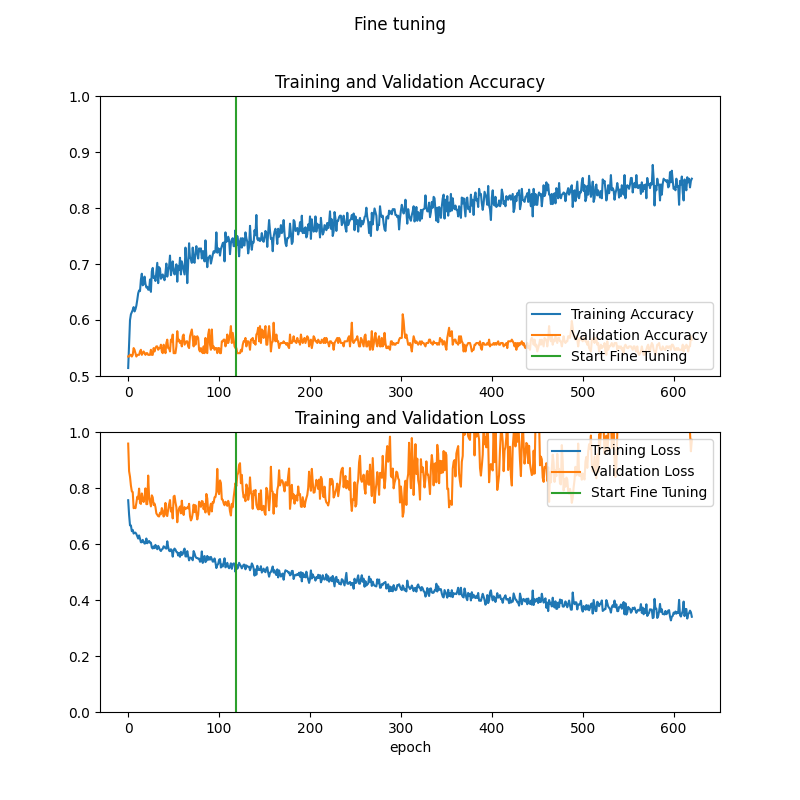
\includegraphics[width=.95\linewidth]{lr10-42_r.png}  
        %\caption{}
        %\label{SUBFIGURE LABEL 4}
    \end{subfigure}
    \caption{Training effettuato con learning rate pari a $10^{-4}$ a seguito dell'augmentation}
    \label{Training Augmentation 2}
\end{figure}
$\\\\$
$\\\\$
Nei grafici precedenti si riporta sia la versione del solo transfer learning che del test comprendente anche
il fine tuning. Nelle seconde figure, per tale motivo si mostra quando inizia il fine tuning (linea verde).
Anche in questo caso la diminuizione della training loss suggerisce il corretto funzionamento nell'allenamento della rete.
Per quanto concerne i risultati ottenuti sono stati riscontrati lievi miglioramenti relativi alla validation accuracy
delle reti, sempre osservando migliori prestazioni da parte della rete con learning rate pari a $10^{-3}$.
Si può infine notare come l'uso della data augmentation ha avuto l'effetto sperato, osservando che la 
validation accuracy dei grafici sopra mostrati non scende.
\chapter{Gestione dati eterogenei}
\label{ch:MLP}
\section{Gestione dei dati}
I risultati ottenuti con la CNN possono essere migliorati o resi più attendibili con l'utilizzo
di altre tipologie di dati. Questi sono le informazioni relative al paziente al momento dell'arrivo in 
ospedale.
\\\\
Tali dati sono di vario tipo, quelli usati dal dataset considerato sono: 
\begin{itemize}
    \item Categorico, esprimono l'appartenenza ad una o più categorie
    \item Booleano, esprimo se il paziente è affetto da una certa patologia o presenta alcuni 
    \item Numerici
\end{itemize}
In questa fase è importante che tutti i dati siano presenti per ogni paziente. Per tale motivo si è dovuto 
trovare un sottinsieme del dataset che presenti il maggior numero di dati. 
\\\\
Per fare ciò sono state eliminate le colonne che non avevano corrispondenze 
tra i pazienti, ovvero erano vuote oppure presentavano dati solo per pochi pazienti.
Al fine di ottenere un risultato migliore sono state eliminati anche i pazienti che non presentavano dati per 
la maggiorparte delle colonne del dataset.
\\\\
Effettuata tale operazione, si è proceduto col creare un unico dataset ottenuto dall'unione 
di training set e test set. Per fare ciò le colonne presenti tra i due devono essere le stesse.
Per tale motivo si è giunti ad un dataset formato dalle seguenti colonne:
\begin{itemize}
    \item Ospedale, dato categorico che rappresenta l'ospedale che ha accolto il paziente tra A,B,C,D,E e F 
    \item Età, dato numerico
    \item Sesso, categorico binario, ovvero maschio o femmina
    \item Tosse, binario
    \item Difficoltà respiratorie
    \item Numero di cellule bianche, dato numerico che indica la percentuale di globuli bianchi nel sangue
    \item Pressione sanguigna alta,  binario
    \item Diabete, binario
    \item Demenza, binario 
    \item BPCO (Broncopneumopatia cronica ostruttiva), binario 
    \item Cancro, binario 
    \item Malattia renale cronica, binario
\end{itemize}
Tali dati sono presenti per 946 pazienti del training set e 472 del test set, per cui abbiamo un dataset di 1218 pazienti.
Questo dataset sarà poi suddiviso in training, validation e test set, per effettuare l'allenamento della rete e per verificare la capacità di effettuare previsioni.
\\\\
Ora che si presenta il dataset completo, si procede col trasformare tutti i dati nello stesso formato, ovvero in valori binari \cite{ar}.
Partendo dai dati categorici, si procede usando la codifica one-hot. Tale procedura prevede che le categorie relative al dato vengano 
trasformate in una rappresentazione binaria, in cui ogni categoria è rappresentata da una serie di zeri ed un unico uno presente nella categoria
codificata.
Per quanto riguarda il sesso, essendo una categoria binaria, si può usare un valore binario, per cui un sesso sarà rappresentato da 0 e l'altro da 1.
L'ospedale è un dato che prevede sei categorie, per cui queste saranno rappresentate da sei bit. Ogni rappresentazione
presenterà cinque zeri ed un unico uno (es. 001000).
\\\\
A livello pratico tali trasfromazioni sono state implementate usando la libreria scikit-learn, in particolare le funzioni
MultiLabelBinarizer(), per l'ospedale, e LabelBinarizer() per il sesso. In tal modo si riesce a trasformare le categorie in array di 
bit, ovvero valori compresi in [0,1].
\\\\
Per gestire i valori numerici si sfrutta un'altra funzione di scikit-learn, ovvero MinMaxScaler().
Tale funzione scala i valori dati in input in un range specificato, nel caso in considerazione [0,1].
La trasformazione avviene mediante:
\begin{equation*}
    \begin{array}{l}
        X_{std} = \dfrac{(X - X.min(axis=0))}  {(X.max(axis=0) - X.min(axis=0))} \\\\
        X_{scaled} = X_{std} * (max - min) + min
    \end{array}
\end{equation*}
\\\\
I valori binari infine sono rimasti invariati, poichè esprimono il valore nel range desiderato.

\section{Struttura MLP}

Avendo ora convertito i dati del dataset in modo da essere in [0,1], si può iniziare a costruire la rete che deve fare previsioni 
prendendo come input tali dati. 
È importante notare che una volta effettuata la codifica one-hot della colonna relativa all'ospedale, si ottiene un vettore di dimensione 6 (una per ogni categoria) al 
posto dell'unica colonna che rappresenta il dato. Per tale motivo la dimensione dell'input della rete non è 
più 12 (in base al numero di colonne presenti inizialmente), ma 17.
\\\\
La rete dunque sarà formata da due layer:
\begin{itemize}
    \item un Dense() layer formato da 30 neuroni
    \item un Dense() layer formato da 5 neuroni
\end{itemize}
Il primo layer è colui che si occupa di ricevere anche gli input, per cui la dimensione degli input dovrà essere pari a 17.
Il secondo layer, invece, è formato da soli 5 layer e si occupa di effettuare una prima classificazione.
Entrambi i layer presentano come funzione di attivazione ReLu.
\\\\
Con tale rete, si riesce dunque ad effettuare il training relativo all'uso dei metadati.

\section{Creazione rete composta}
Per poter usare contemporaneamente le due reti neurali create, ovvero la CNN e la MLP, si necessita di 
un ulteriore passaggio.
Lo scopo di tale passaggio è avere una rete che accetti come input sia immagini che i metadati relativi, al fine
di ottenere una previsione più affidabile, poiché basata sull'uso di più dati.
\\\\
Per gestire gli output delle due reti questi vengono concatenati, in modo da ottenere un unico array di output.
Al fine di effettuare le predizioni su tale output si aggiunge, alla fine della rete, un ulteriore 
Dense layer, formato da un unico neurone, con funzione di attivazione Sigmoid e che prende un input della 
dimensione della combinazione degli output delle due reti. 
\\\\
Si può, infine, creare la rete che prende in input la combinazione degli input della rete, mentre l'output sarà determinato
dal nuovo layer inserito.
*immagine rete completa*
Ora si può dunque procedere con la compilazione della rete e con il training.  
%\chapter{Risultati}
\label{ch:MLP}
\section{Risultati ottenuti}


%%%%%%%%%% APPENDIX %%%%%%%%%%%%%%%%%%%

%\appendix
%\chapter{Appendice}
%%%%%%%%%% CONCLUSIONI %%%%%%%%%%%%%%%%%%%
\chapter*{Conclusioni}
\chaptermark{Conclusioni}
\addcontentsline{toc}{chapter}{Conclusioni}
In questo progetto di tesi si è focalizzata l'attenzione sull'uso dei reti neurali convoluzionali e di percettrone multistrato per analizzare ed effettuare 
previsioni usando un dataset fornito.
Il dataset si può suddividere nelle immagini, raffiguranti radiografie del torace, e nei metadati relativi alle immagini.
\\\\
In primo luogo si è compreso la composizione del dataset, si è osservato che le immagini avevano dimensioni varie e presentavano alcune differenze a livello 
di luminosità dell'immagine. Per tali motivi sono stati effettuati alcuni accorgimenti per migliorare la qualità delle immagini e ridimensionarle.
\\\\
In tal modo si è migliorata la qualità del dataset. Per procedere con il training della rete convoluzionale, si è dovuto prima creare immagini in cui si vedono solamente i polmoni.
Tale passaggio sfrutta la U-Net per individuare la collocazione dei polmoni nell'immagine.
\\\\
Una volta termimnato questo studio sullle immagini si è passato al training vero e proprio della rete convoluzionale.
Per migliorare le prestazioni della rete sono stati applicate le tecniche di Fine Tuning e Transfer Learning.
Alla fine si è proceduto con l'effettuare dei training di test e i risultati ottenuti sono stati analizzati.
\\\\
Per l'implementazione dell'MLP si è deciso di usare dei layer che calcolano l'output partendo da un insieme di metadati presi dal dataset.
Anche in tal caso sono stati effettuati accorgimenti sul dataset, in modo da avere un suo sottinsieme completo, poiché erano presenti dati mancanti.
\\\\
In fine è stata creata un unica rete, composta dalle precedenti in modo che possa prendere in ingresso sia immagini che metadati e restituire un risultato più accurato.
\\\\
Una modifica interessante del lavoro effettuato è rendere il modello utilizzabile su dataset che presentano dati mancanti.
In alternativa si potrebbero comparare le prestazioni ottenute con reti differenti.
%%%%%%%%%% Ringraziamenti %%%%%%%%%%%%%%
%%%%%%%%%% BIBLIOGRAPHY %%%%%%%%%%%%%%
\phantomsection
\printbibliography[heading=bibintoc]

%%%%%%%%%%%%%%%%%%%%%%%%%%%%%%%%%%%%%%

\end{document}